% !TeX root = ../main.tex
% Add the above to each chapter to make compiling the PDF easier in some editors.


\chapter{Introduction}\label{chapter:introduction}

An important topic in computer science is the study of the
\textit{functional correctness} of an algorithm.
It states whether an algorithm satisfies specified
input/output behavior.
Proving an algorithm correct
becomes especially interesting when a) it can be applied
to directly executable code and b) it is machine checked.
Unfortunately with both desirable additions, the task becomes
significantly more complex.
Even in an abstract specification, where topics such as
memory management may be abstracted away,
machine checked proofs of non-trivial properties
are hard.
Furthermore for concrete implementations,
low-level decisions about memory allocation or
the eligibility of reusing variables need to be
reasoned about.
In this thesis we provide a computer assisted proof in the interactive
theorem prover Isabelle/HOL for the functional
correctness of an imperative implementation of the B-tree data-structure
and present how we dealt with the above mentioned issues.

In \Cref{chapter:introduction}, we have a brief overview on related
work and introduce common variations of the definition of B-trees.
We choose to implement the definition that is most promising for our approach.
We first design a functional, abstract implementation.
Together with a proof of its functional correctness,
it is presented in \Cref{chapter:abs-set}.
On this level, functional correctness means that we show the specifications
implement an abstract set interface for linearly ordered element.
This interface supports membership queries as well as insertion and deletion operations.
From the functional specification, an imperative implementation is derived in \Cref{chapter:imp-set}.
Its functional correctness is shown by proving that it refines the functional specification.
Thus the proof obligation for the imperative implementation
is reduced to a proof of equivalence between the output of the
functional and the imperative implementation.
This allows for low-key optimizations with regard to a naive translation.
Finally, we present learned lessons, compare the results with related work and suggest potential future
research in \Cref{chapter:conclusion}.

% TODO related work?
% mfp/fielding: not mechanized, different approaches
% Ernst: more automation, but actually similar approach to ours (except for used structure)
% Malecha: less automation, similar structure


\section{The Isabelle Proof Assistant}

Isabelle/HOL is an interactive theorem prover that allows
to reason, among other things,
in Higher Order Logic \parencite{DBLP:books/sp/NipkowPW02}.
It is built in ML, which influences the syntax of functional
programs written in it.
Isabelle source files are divided in so called theories,
corresponding to code modules in common programming languages.
A theory consists of the specification of datatypes,
typed definitions and theorems with proofs.

\subsection{Notation and proofs in Isabelle}

Functions, predicates and the like are all expressed in
a functional manner.
The keyword \textbf{definition} denotes classical definitions.
The term \textbf{abbreviation} is used to define simple shorthands for more complex expressions,
similar to a macro.
The word \textbf{fun} precedes recursively defined total functions.
It supports definition by pattern matching and
is only a valid definition if it incorporates a proof of termination.
Usually this proof is derived automatically by the system.
If a termination can not be guaranteed for all inputs,
a function may be defined via \textbf{partial\_function}.
As circle free-ness of heap pointers cannot be guaranteed for all inputs
on imperative programs, many imperative definitions are given
as partial functions.
Partial function definitions come at the inconvenience of no
supported pattern matching \parencite{isabelleManual}.

Lemmas, theorems and the like can be expressed in a similar manner
as they would be written in mathematical textbook.
They begin with \textbf{lemma}, \textbf{theorem} or \textbf{corollary},
followed by an expression or predicate and a proof.
Wherever possible and readable, we will try to reflect the actual
syntax of the Isabelle system, however compromise in order to
keep the notation of obtained lemmata and theorems
close to conventional notation.
To prove a theorem correct, the system basically provides two different
proof styles.

One option is to write structured proofs in the isar language.
The user outlines a proof with intermediate goals
and tells the system which proof methods to apply to
resolve each step.
This method is usually preferred as it is more readable and usually
faster on the system side.
All complex proofs in \Cref{chapter:abs-set} are hence written in this style.

In the apply style, the user tells the system which proof method
to apply to modify the current goal.
Examples are the application of a rule
or simplification using equivalences.
This is practical if the number of assumptions
is high or the goal is large and writing the full terms
out would be impractical.
Since this is the case for the proofs of the imperative programs,
almost all proofs in \Cref{chapter:imp-set} are written in this style.

The system provides a number of proof methods,
based on different manipulation tools
such as logical reasoning or simplification.
In this work we will not present the proofs as written in the actual
proof files but rather outline the structure of the proofs.
When mentioning \textit{automatic} proofs, we mean a proof that
comprises very few ($\le 5$) apply style
invocations of proof methods.
A method that commonly allows for such proofs is the \textit{auto} method,
a combination of logical reasoning and repeated simplification,
but also allowing automatic case distinctions and destructive rule application.

It is possible to specify functions, predicates
and theorems with respect to some abstracted function or constant
on which only certain assumptions are made,
resulting in so-called \textbf{locales}.
By providing functions or constants that satisfy
the assumptions, we may \textit{instantiate}
the locale.
We implement the set interface concretely by
instantiating a set locale from the standard library.

\subsection{Examples and basics of the Isabelle language}

Datatypes may be defined recursively.
The following shows as an example the internal definition of the list datatype.\footnote{
    The actual definition is worded slightly different but this is of no importance here.
}

\begin{lstlisting}[mathescape=true, language=Isabelle,label=lst:list-def]
datatype 'a list = [] | 'a # 'a list
\end{lstlisting}

In natural language this means that either a list is the empty list,
or it is an element prepended to another list.
As usual in ML like languages, we may apply pattern matching to function argument.
In addition, the type $'t$ of any expression $e$ can be
made explicit by writing \textit{e :: 't}.
Functions that take values of type $'a$ and return values of type $'b$ 
have type \textit{'a $\Rightarrow$ 'b}.
For functions that take several arguments,
currying is applied.
The Isabelle internal list catenation function "@" serves as
an example for a function definition with explicit type.

\begin{lstlisting}[mathescape=true, language=Isabelle,label=lst:append-def]
fun (@) :: 'a list $\Rightarrow$ 'a list $\Rightarrow$ 'a list where
    [] @ ys = ys |
    (x#xs) @ ys = x # (xs @ ys)
\end{lstlisting}

% TODO include?
% locales
% set specification

Further details on notation, proof techniques and more in Isabelle/HOL
may be found in Chapter 1 of \parencite{DBLP:books/sp/NipkowK14}.


\section{The B-Tree Data Structure}

B-trees were first proposed by Bayer in \parencite{DBLP:journals/acta/BayerM72},
as a data-structure to efficiently retrieve and manipulate
indexed data stored on storage devices with slow memory access.
They are $n$-ary balanced search trees.
As such B-trees are generally said to implement a map interface,
mapping indices to data and supporting map updates and deletions.
They may also be specified as implementing a set interface,
where the indices form the actual content of the set.
B-trees are a generalization of 234-trees and a specialization of (a,b)-trees.

A commonly implemented variation is the B$^+$-tree, where the inner nodes
only contain separators to guide the recursive navigation through the tree.
In B$^+$-trees, all data is stored in the leaves \parencite{DBLP:journals/csur/Comer79}.
Further the leaves are often implemented so as to contain pointers
to the next leaf in order, allowing for efficient range queries.

Node are generally thought to be implemented by
containing a number of indices, corresponding data and children.

\subsection{Definitions}
\label{sec:data_structure_defs}

Every node contains a list of \textit{keys} (also \textit{separators}, \textit{index elements}), and \textit{subtrees} (\textit{children}),
that represent further B-tree nodes.
The separators and subtrees may be considered interleaved within a node,
such that we can speak of a subtree left of a separator and a subtree right of a separator,
where for a separator at index $i$ we mean the subtree in the respective
subtree list at index $i$ and $i+1$ respectively.
Note that this already implies that the list of subtrees is one
longer than the list of separators - we refer to the last subtree
as the \textit{last} or \textit{dangling} subtree.
In the original definition by Bayer \parencite{DBLP:journals/acta/BayerM72},
a B-tree with above structure must fulfill the three properties
\textit{balancedness}, \textit{order} and \textit{sortedness}.

\paragraph{Balancedness} \textit{Balancedness} requires
that each path from the root to any leaf has the same length $h$.
In other words, the height of all trees in one level of the tree must be equal,
where the height is the maximum path length to any leaf.
It is only possible to maintain this property
due to the flexible amount of subtrees in each node.

\paragraph{Sortedness} Further the indices must be \textit{sorted} within the tree which means that all indices stored
in the subtree left of a separator are smaller than the value of the separator
and all indices on the right are greater.
Further all indices within a node should maintain a sorted order,
that is the list of separators in a node must be sorted.

\paragraph{Order} In general terms, the property of \textit{order} ensures a certain minimum and maximum
number of subtrees for each node.
However, as pointed out by Folk and Zoellick \parencite{DBLP:books/daglib/0095349_mod},
the property is defined differently in the literature.
For the purpose of this work, the original definition by Bayer
was chosen as most suitable.
A B-tree is of order $k$, if each internal node has at least $k+1$
subtrees and at most $2k+1$.
The root is allowed to have a minimum of 2 subtreess and a maximum of $2k+1$.

An alternative definition proposed by Knuth \parencite{DBLP:books/lib/Knuth98a},
is to allow between $\lceil \frac{k}{2} \rceil$ and $k$ children.
However this involves cumbersome \textit{real} arithmetic that unnecessarily complicates
mechanized proofs.
Sticking to the original definition is further supported by the fact that nodes are supposed
to fill memory pages which are usually of even size (usually some power of 2).
An even number of separators and trees plus one dangling last right tree maximizes
the usage of such a page.

The same ambiguity exists for the term \textit{Leaf} which we will define consistently with Knuth's definition \parencite{DBLP:books/lib/Knuth98a}
to be an empty node, carrying no information,
rather than a node that contains data but no children.
This is close to the usual approach in functional programming,
and will yield more elegant recursive equations for our B-tree operations.
The lowest level of nodes hence contains a list of separators and
list of pointers to leaves as can be seen in \Cref{fig:btree-basic-nopair}.

Note that the B-tree definition is only meaningful for positive $k$.
For the case that $k$ is equal to 0,
all elements of the tree would have exactly one subtree
and no internal elements.
For the root node this even leads to a contradictory state:
It is required to contain at least 1 element or 2 subtrees.
However as it should not have more than $2k+1 = 1$ elements,
this constraint cannot be satisfied.
Requiring positive $k$ is consistent with the definitions
in the consulted literature \parencite{DBLP:journals/acta/BayerM72,DBLP:journals/csur/Comer79,DBLP:books/daglib/0023376}.

% insert image of valid B-tree

\begin{figure}
    \centering
    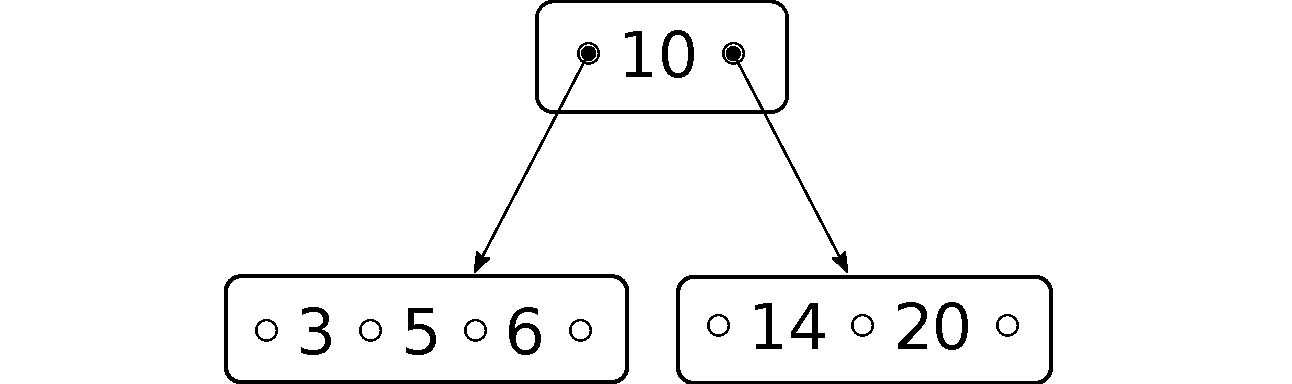
\includegraphics[width=0.5\linewidth]{figures/btree-basic-nopair.pdf}
    \caption[A small example B-Tree]{A small balanced, sorted B-tree of order $2$ and
    height $2$ containing $3$ nodes and $6$ elements.
    In subsequent depictions, leafs will be depicted
    by empty circles.}
    \label{fig:btree-basic-nopair}
\end{figure}

\subsection{B-Tree operations}

The B-tree is a dynamic data-structure and provides
a number of operations to inspect or modify the stored data.
Generally, the operations are defined recursively on the nodes.
The correct subtree may be found by inspecting the separators stored
in the currently visited node.
If the value that is being searched for is in the range of two
adjacent separators and equal to neither of them,
we recurse into the tree in between. 
The obvious corner cases are if the value is less than the
minimal element or greater than the maximum element stored.
In that case we recurse in either the first or the last subtree.
The exact manner of inspection should in practice of course
be efficient and will hence be kept abstract until \Cref{chapter:imp-set}.

\paragraph{Retrieval}\label{par:intro-isin}
Since the whole tree is sorted,
checking whether certain elements are contained in the tree
is simply conducted by recursing into the correct node
in each level.
Either the element is found directly or found at a lower level.
If we reach a leaf node we know that the element is not contained in the tree.
There is little variation on this algorithm so there is no need for comparison.

% TODO move abstract discussion to introduction
%-------------------------------------------------
\paragraph{Insertion}\label{par:intro-ins}
There is also much consensus in the literature on
how to conduct insertion into a B-tree \parencite{DBLP:journals/csur/Comer79}.
%TODO citations
%TODO relationship to other implementations (are there more?)
Generally, an element is inserted into the nodes on the lowest level.
In a first step, the element is simply placed at the correct
position in the list of separators.
If the node had enough space left prior to this operation,
we are done.
If however the node has more than $2k$ elements after this insertion,
we need to split it and, passing the median to the parent node,
recurse back upwards.
We will see in \Cref{sec:abs-ins} how this can be
elegantly expressed in a functional specification.
More detailed descriptions and examples of insertion and deletion may be found
in \parencite{DBLP:books/daglib/0023376}.
%-------------------------------------------------

% TODO delete
% TODO move abstract discussion to introduction
%-------------------------------------------------
\paragraph{Deletion}\label{par:intro-del}
On deletion, elements are removed from the leaves only.
If the element to be deleted resides in an inner node,
it is replaced by the maximal lesser or minimal greater
element in the tree, which always resides in a leaf
to the left or right of the element to be removed.

After deletion, the nodes may need rebalancing in order
to ensure the order property.
A node having less than $k$ elements is called to have \textit{underflow}.
Opposing to the insertion function,
the exact procedure to handle underflow varies strongly in the literature.
Since only one element is removed from the node,
the most intuitive remedy to underflow is to \textit{steal} or \textit{borrow} it
from the left or right sibling \parencite{DBLP:books/daglib/0023376}.
If the left or right sibling has more than $k$ elements,
one of the neighboring elements may be moved into the current node.
Only in case that both siblings have left only $k$ elements,
a kind of reversal of the insertion split is conducted:
One of the siblings and the node itself, together with the separating
element of the parent node are merged and the result split again to form
a new, bigger node of valid order.

Following the description of Bayer \parencite{DBLP:journals/acta/BayerM72},
as done by Fielding \parencite{Fielding80},
the two cases can be treated identically.
If a node has less than $k$ elements,
merge it with one of its siblings.
If the resulting catenated node has an overflow again,
it will be split in half, just as with insertion related overflows.
According to Comer \parencite{DBLP:journals/csur/Comer79} this may even be
more efficient than stealing single single keys from siblings.
First of, the resulting node is less likely to underflow again.
If it had stolen only one element, the probability for another underflow at the next
deletion from this node is 1, higher than if several elements are copied over.
Further, the node to merge with been completely read from memory at the point
of stealing an element.
Merging does therefore not incur additional memory accesses and
the cost of inter-memory copy of up to $k$ elements is negligible.

%-------------------------------------------------

\subsection{Properties}

B-trees are assumed to be stored on external memory,
such that each node roughly matches a page in main memory.
Due to the potentially large branching factor and the balancing,
the number of required memory accesses for retrieving data stays small even for
large amounts of data stored.
This is due to the fact that the overall number of memory accesses is bounded by the depth
of the tree, which again is logarithmic in the number of indices -
where the base of the logarithm is closely proportional to the order $k$ of the tree.

Further, by design, the storage usage of B-trees is at a minimum close to $50\%$,
where the average usage is usually higher \parencite{DBLP:journals/acta/BayerM72}.
This is achieved by ensuring that every node reserves the storage of $2k$ keys and separators.
By definition, the nodes (except for the root) always contain
at least $k$ elements, yielding a storage usage of close to $50\%$.

B-trees lay the foundation to most modern relational database implementations.
The above mentioned properties are key to the widespread popularity of B-trees
in databases and are hence preserved in the given implementation.
% TODO more

\section{Related Work}

All found related work considers B$^+$-trees
rather than B-trees, however some parallels can be found.

There exist two pen and paper proofs via the rigorous approach
by Fielding \parencite{Fielding80} and Sexton \parencite{DBLP:journals/entcs/SextonT08}.
Even though not machine checked, they shed light on techniques applied in this work.

Fielding approaches the verification by refinement.
First, B$^+$-trees are viewed as nested sets of subtrees
or as leafs that are sets of key-value pairs.
Obtaining the correct subtree for recursion is in the abstract setting
only defined by appropriate pre and post-condition
and an actually executable function is provided in the second refinement step.
On this level, only arguments on the invariants are made.
In a second step B-trees are considered more concretely to contain
sorted lists of children and keys.
Here the argument for invariant preservation is due to the implementation
having the same structure as the implementation in the abstract context.
Final imperative PASCAL code is given, derived by hand
imitating the functional style implementations and extended by assertions.

This approach is similar to what will be done in this work,
however mostly concerning the methodology rather than the actual
steps of refinement.
In this work, we will start at the definition using lists in \Cref{chapter:abs-set}
and refine to an imperative implementation with pointers and arrays in \Cref{chapter:imp-set}.
The code we obtain will be exported automatically to a functional language of choice.

We reason about the validity of this refinement via separation logic,
the same tool as employed by Sexton \parencite{DBLP:journals/entcs/SextonT08}.
They show in their work that this tool allows to reason based on some kind of locality,
in particular that operations on subtrees are really only affecting subtrees.
We will make implicit use of this property in \Cref{chapter:imp-set}
for proofs on our imperative implementation.

The specification by Sexton is given as an abstract machine rules,
somewhat more abstract than pure code but operating on a stack
much like we expect imperative programs to operate with pointers on a heap.
We therefore categorize this as a direct proof on an imperative implementation.

Of these imperative implementations, also two machine checked proofs exist.
In the work of Ernst \parencite{DBLP:journals/sosym/ErnstSR15},
an imperative implementation is directly verified
by combining interactive theorem proving 
with shape analysis.
The main recursive procedures are interactively verified in KIV.
Data structure properties such as circle-freeness are then proven by shape-analysis.
Another direct proof on an imperative specification 
was conducted by Malecha \parencite{DBLP:conf/popl/MalechaMSW10}, with the YNOT
extension to the interactive theorem prover Coq.
Both works use recursively defined "shape" predicates
that describe how the nodes and pointers
form a bounded and circle free abstract tree.
However, we know of no verification that explicitly covers
the implementation of functional B-trees.
In addition to providing one, this work aims to show the benefits
of taking this indirection for imperative implementations.
That is that the analysis of invariants of an abstract shape may be spared
or at least significantly simplified when
restricting the concrete pointer structures to be refinements
of an abstract algebraic type.